\begin{theo}[Arbeid en energie]{Arbeid en energie}

    Arbeid is een scalaire grootheid voor het energietransfert, andersom is energie dan een scalaire grootheid voor de capaciteit om arbeid te leveren.

    \begin{itemize}
    
        \item{Arbeid en energie door een constante kracht}
        
            De arbeid geleverd door een constante kracht is gelijk aan de volgende formule:
            \begin{equation*}
                W = F_{||}d = Fdcos(\theta) = \Vec{F} \cdot \Vec{d}
            \end{equation*}
            \begin{center}
                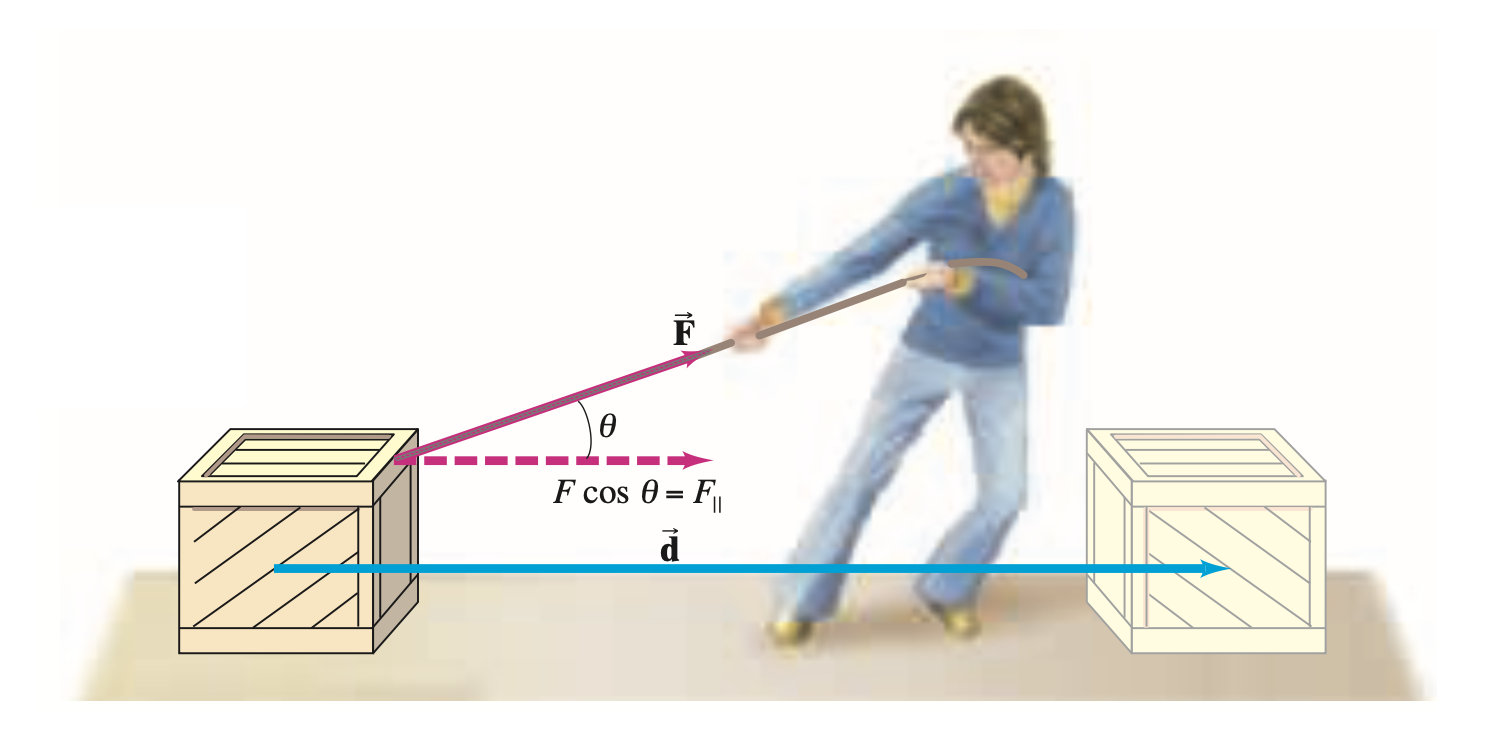
\includegraphics[scale = 0.15]{Images/Dynamica/Arbeid bij constante kracht.png}
            \end{center}
        \item{Arbeid en energie door een variabele kracht}
        
            Stel het voorwerp wordt bewogen door een variabele kracht over een pad $ a \to b $. We kunnen dit pad opsplitsen in infinitesimalen delen $ d\Vec{\ell} $. Als we nu integreren over het pad, dan krijgen we: 
            \begin{equation*}
                W = \int_{a}^{b}  F_{||}d\ell = \int_{a}^{b} F \cos\theta d\ell = \int_{a}^{b} \Vec{F} \cdot d\Vec{\ell}
            \end{equation*}
    \end{itemize}
\end{theo}

\begin{app}[Terugroepkracht van schroefveren]{Terugroepkracht van schroefveren}
    
    \begin{minipage}{.68\textwidth}
    
    Het uittrekken of samendrukken van een veer veroorzaakt een kracht, namelijk de terugroepkracht: 
    
    \begin{equation*}
        \Vec{F}_s = -k\Vec{x}
    \end{equation*}
    
    De arbeid geleverd door de veer hangt kunnen we ook berekenen:
    
    \begin{equation*}
        W_s = \int_0^x \Vec{F}_s \cdot d\Vec{x} = -\dfrac{1}{2}kx^2
    \end{equation*}

    Deze zal gelijk zijn bij samendrukken en uitrekken. \\

    \textbf{Opmerking}: de formule is geldig als de massa begint in de oorsprong en samengedrukt/uitgerokken wordt tot een punt x
    
    % Hieruit volgt dus ook dat $ W_{net} = 0 $ als we van $ -x \to x $, want:
    
    % \begin{equation*}
    %     W_{net} = W_{s,uit} + W_{s,sam} = -\dfrac{1}{2}kx^2 + \dfrac{1}{2}kx^2 = 0
    % \end{equation*}
    
    \end{minipage} 
    \begin{minipage}{.32\textwidth}
    
        \centering
        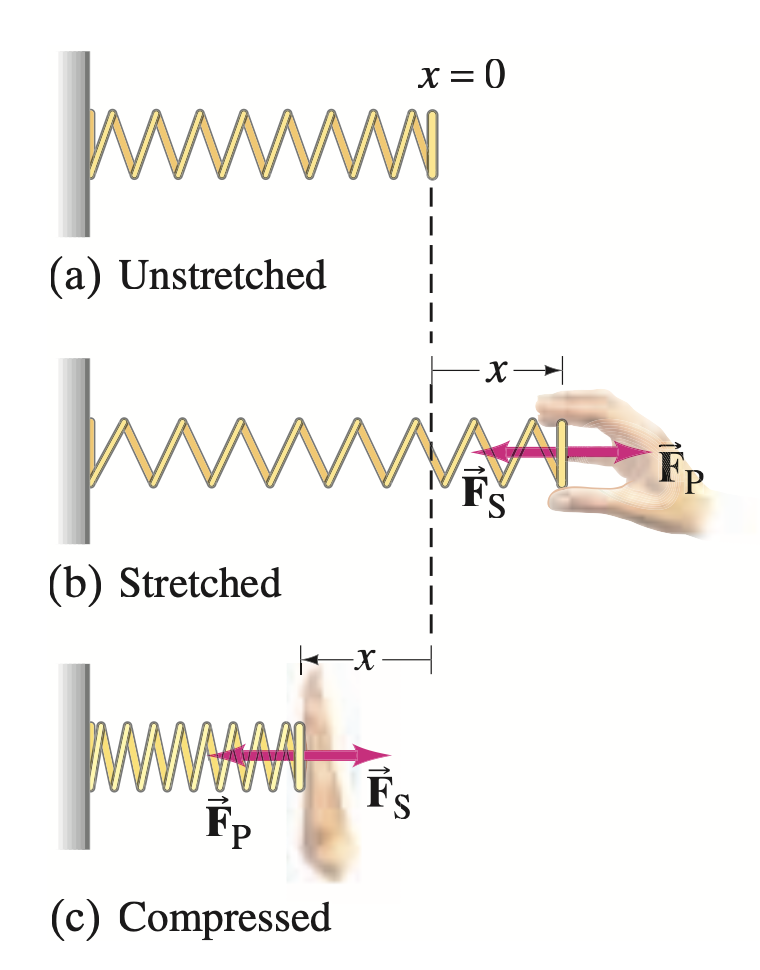
\includegraphics[scale = 0.325]{Images/Dynamica/Schroefveer.png}
        
    \end{minipage}
\end{app}

\begin{lem}[Arbeid - Kinetische energie theorema]{Arbeid Kinetische energie theorema}

De netto-arbeid $ W_{net} $ geleverd door een voorwerp wordt bepaald door de netto-kracht $ F_{net} $. Stel we hebben een variabele (of een constante) kracht die inoefent op een voorwerp, we berekenen nu de netto-arbeid: 

\begin{align*}
    W_{net} &= \int_i^f \Vec{F}_{net} \cdot d\Vec{\ell} \\
            &= \int_i^f F_{||}d\ell \\
 \hspace{6.5cm} &= \int_i^f m\dfrac{dv}{dt}d\ell \qquad \qquad \ \ (F_{||} = ma_{||} = m\dfrac{dv}{dt}) \\
            &= \int_i^f mvdv \qquad \qquad \quad \  (v=\dfrac{d\ell}{dt}) \\
\hspace{6.5cm} &= \dfrac{1}{2}mv_f^2 - \dfrac{1}{2}mv_i^2 \quad \quad (F_{net} = ma, \ a = \dfrac{v_2^2 - v_1^2}{2d}) \\ 
            &= \Delta K 
\end{align*}

\noindent Wat we hierboven bewezen hebben is het \textbf{Arbeid - Kinetische energie theorema}, in woorden: 

\vspace{0.3cm} \noindent  `Wanneer de enige verandering in het systeem de snelheid is, dan is de arbeid verricht door de nettokracht gelijk aan de verandering in kinetische energie van het systeem.`

\end{lem}
